\documentclass{article}
\linespread{1.3}
\usepackage[margin=50pt]{geometry}
\usepackage{amsmath, amsthm, amssymb, amsthm, tikz, fancyhdr}
\pagestyle{fancy}
\renewcommand{\headrulewidth}{0pt}
\newcommand{\changefont}{\fontsize{15}{15}\selectfont}

\newcommand{\field}[1]{\mathbb{#1}}
\newcommand{\1}{\mathbf{1}}
\newcommand{\E}{\mathbb{E}} 
\renewcommand{\P}{\mathbb{P}}
\newcommand{\R}{\field{R}} % real domain
% \newcommand{\C}{\field{C}} % complex domain
\newcommand{\F}{\field{F}} % functional domain

\newcommand{\T}{^{\textrm T}} % transpose

\def\diag{\text{diag}}

%% operator in linear algebra, functional analysis
\newcommand{\inner}[2]{#1\cdot #2}
\newcommand{\norm}[1]{\left\|#1\right\|}
\newcommand{\twonorm}[1]{\|#1\|_2^2}
% operator in functios, maps such as M: domain1 --> domain 2
\newcommand{\Map}[1]{\mathcal{#1}}
\renewcommand{\theenumi}{\alph{enumi}} 

\newcommand{\Perp}{\perp \! \! \! \perp}

\newcommand\independent{\protect\mathpalette{\protect\independenT}{\perp}}
\def\independenT#1#2{\mathrel{\rlap{$#1#2$}\mkern2mu{#1#2}}}
\newcommand{\vct}[1]{\boldsymbol{#1}} % vector
\newcommand{\mat}[1]{\boldsymbol{#1}} % matrix
\newcommand{\cst}[1]{\mathsf{#1}} % constant
\newcommand{\ProbOpr}[1]{\mathbb{#1}}
\newcommand{\points}[1]{\small\textcolor{magenta}{\emph{[#1 points]}} \normalsize}
\date{{}}

\fancypagestyle{firstpageheader}
{
  \fancyhead[R]{\changefont Michael Huang \\ CSE 446 \\ Homework 2}
}

\begin{document}

\thispagestyle{firstpageheader}

\section*{A.0}
{\Large 

\framebox[1.1\width]{\textbf{answer}}

\subsection*{a.}

Suppose that your estimated model for predicting house prices has a large positive weight on the feature \texttt{number of bathrooms}. If we remove this feature and refit the model, will the new model have a strictly higher error than before? Why? \\ \\

% is this pre/post regularization
If we removed this feature that had large positive weight and refit the model, then the new model wil not necessarily have strictly higher error than before. It is difficult to say that there is a distinct 

\subsection*{b.}

Compared to L2 norm penalty, explain why a L1 norm penalty is more likely to result in sparsity (a larger number of 0s) in the weight vector. \\ \\ 

An L1 norm penalty is more likely to result in sparsity in the weight vector since it will linearly decrease towards 0 with each step, which means that it will actually reach 0, which is not the case with the quadratic steps towards 0. L1 is therefore more likely to zero out coefficients.

\subsection*{c.}

In at most one sentence each, state one possible upside and one possible downside of using the following regularizer:$\left(\sum_{i}\left|w_{i}\right|^{0.5}\right)$ \\ \\
One possible upside is that it is that features will tend to be zeroed out less often, which maintains these features' input in the model. \\ 
One possible downside is that weights will tend to be larger for features that are less relevant, since we don't get as large gradients and changes when we perform regularization, especially when we near zero.
% all the weights will tend to be less sparse.

\subsection*{d.}

True or False: If the step-size for gradient descent is too large, it may not converge. \\ \\

True; if the step-size for gradient descent is too large, then it may diverge. This is because with a step size that is too large, then the values may oscillate around an optimal point rather than generally converge upon it, as it would with more common algorithms.

\subsection*{e.}

In your own words, describe why stochastic gradient descent (SGD) works, even though only a small portion of the data is considered at each update. \\ \\

Stochastic gradient descent iteratively chooses random samples from training data to update parameters. By randomly approximating the distribution dataset around the chosen random sample, we can effectively guess the gradients and update the weights based on the attributes of the distribution each time rather than having to run through all the data.

\subsection*{f.}

In at most one sentence each, state one possible advantage of SGD over GD (gradient descent), and one possible disadvantage of SGD relative to GD. \\ \\

SGD might be better than GD since you don't need to run through all samples in a set of training data, and save time overall. \\ 
% often converges much faster
SGD might be worse than GD since the error might not be as well minimized.\\

}

\section*{A.1}
{\Large

A \emph{norm} $\|\cdot\|$ over $\R^n$ is defined by the properties:
(\textit{i}) non-negativity: $\|x\|\geq 0$ for all $x \in \R^n$ with equality if and only if $x=0$,
(\textit{ii}) absolute scalability: $\|a \, x\| = |a| \, \|x\|$ for all $a \in \R$ and $x \in \R^n$, 
(\textit{iii}) triangle inequality: $\|x+y\| \leq \|x\| + \|y\|$ for all $x,y \in \R^n$. \\ \\

Context: norms are often used in regularization to encourage specific behaviors of solutions. If we define  $\| x \|_p := \left( \sum_{i=1}^n |x_i|^{p} \right)^{1/p}$ then one can show that $\| x \|_p$ is a norm for all $p \geq 1$. The important cases of $p=2$ and $p=1$ correspond to the penalty for ridge regression and the lasso, respectively.

\subsection*{a.}

We aim to prove that $f(x) = \left( \sum_{i=1}^n |x_i| \right)$ is a norm. \\ \\
$(i)$ We start with showing non-negativity. \\
We first take the absolute value for each $x_i$ contained within $x$, and we know that \\
$|x_i| \geq 0$ $|_{i = 1, \dots, n}$ \\
We also know that the sum of non-negative elements will also be non-negative, which in turn tells us that \\ 
$\sum_{i=1}^{n} |x_i| \geq 0$ \\
We also need to show that if and only if $x = 0$, $\|x = 0\|$. \\
First, we know that if $x = 0$, then $|x| = 0$ as we know that since each $x_i = 0$,  \\
$|x_i| = |0| = 0$ $|_{i = 1, \dots, n}$ \\
which in turn tells us that \\ 
$\sum_{i=1}^{n} |x_i| = \sum_{i=1}^{n} |0| = 0$ \\
Then, we need to show the other direction; that is, if and only if $\|x\| = 0$, $x = 0$. By the contrapositive, we can say that if $x \neq 0$, then $\|x\| \neq 0$. If $x \neq 0$, then we know that as we now know through absolute value, \\
$|x_i| > 0 |_{i = 1, \dots, n}$ \\
which in turn using addition tells us that  \\ 
$\sum_{i=1}^{n} |x_i| > 0 \neq 0$ \\
which is exactly what we sought to show. \\ \\
$(ii)$ We then look at absolute scalability. By definition, \\
$\|ax\| $ \\
$ = (\sum_{i=1}^{n} |ax_i|)$ \\
$ = (\sum_{i=1}^{n} |a| |x_i|)$ \\
$ = (|a| \sum_{i=1}^{n} |x_i|)$ \\
$ = |a| (\sum_{i=1}^{n} |x_i|)$ \\
$ = |a| \|x\|$ \\
which is exactly what we sought to show. \\ \\
$(iii)$ Finally, we look at the triangle inequality. We begin by showing that $|a + b| \leq |a| + |b|$ for all $a, b \in \R$: \\
$|a + b| \leq |a| + |b|$ \\
$(|a + b|)^2 \leq (|a| + |b|)^2$ \hfill Square both sides \\
$a^2 + b^2 + 2ab \leq a^2 + b^2 + 2|a||b|$ \\
$2ab \leq 2|ab|$ \\
$ab \leq |ab|$ \\ 
We can see that this statement is true since if $a$ and $b$ are both positive or both negative, then the two sides are equal. However, in the case that $a$ and $b$ are of opposite signs, then we can see that although the magnitudes of both sides will be equal, the left side will be negative, and the right side will be positive, which makes the left side less than the right side. \\
We can then go on to use this in proving the statement: \\
$\|x + y\| $ \\ 
$= (\sum_{i=1}^{n} |x_i + y_i|) $ \\
$\leq (\sum_{i=1}^{n} |x_i| + |y_i|) $ \hfill Using what we proved \\
$\leq (\sum_{i=1}^{n} |x_i| + \sum_{i=1}^{n} |y_i|) $ \\
$\leq (\sum_{i=1}^{n} |x_i|) + (\sum_{i=1}^{n} |y_i|) $ \\
$\leq \|x\| + \|y\|$ \\
which is exactly what we sought to show. \\ \\
Since we have proved that all 3 properties hold for $f(x)$, we can see that it is indeed a norm. 

\subsection*{b.}

We aim to show that $g(x) = \left(\sum_{i=1}^n |x_i|^{1/2}\right)^2$ is not a norm, which we can easily show using a counterexample. If we take two $n=2$ dimensional plants $x = (1, 9)$ and $y = (16, 0)$, we see that the triangle inequality does not hold: \\
$\| x \| = (|1^{1/2}| + |9^{1/2}|)^2 = (1 + 3)^2 = 4^2 = 16$ \\ 
$\| y \| = (|16^{1/2}| + |0^{1/2}|)^2 = (4 + 0)^2 = 16$ \\ \\
$\|x + y\| \leq \|x\| + \|y\|$ \\ 
$((1 + 9)^{1/2} + (16 + 0)^{1/2})^2 \leq 16 + 16$ \\ 
$(\sqrt{10} + 4)^2 \leq 32$ \\ 
$10 + 16 + 8\sqrt{10} \leq 32$ \\ 
$26 + 8\sqrt{10} \leq 32$ \\ 
$\sim 51.30 \leq 32$ \\ 
which is false and shows that the triangle inequality does not hold, which tells us that $g(x)$ is indeed not a norm.

}

\section*{A.2}
{\Large 

\subsection*{I}
Not convex. We see that connecting point $b$ to $c$ results in a line outside of the grey shaded set.

\subsection*{II}
Convex. We see that any line that we draw between points stays within the shaded set.

\subsection*{III}
Not convex. We can see that connecting point $d$ to $a$ would result in a line outside of the grey shaded set.

}

\section*{A.3}
{\Large 

\subsection*{a.}

The function is convex, as we see that any connections between points are contained above the function.

\subsection*{b.}

The function is not convex. It is possible to connect lines between points that are below the function, such as from point $a$ to $b$ or from point $b$ to $c$.

\subsection*{c.}

The function is not convex. It is possible to connect lines between points that will have sections below the function, such as from point $a$ to any other point on the interval.

\subsection*{d.}

The function is convex, since any connections between points would be constructed above the function.

}

\section*{A.4}
{\Large 



\subsection*{a.}

With your synthetic data, solve multiple Lasso problems on a regularization path, starting at $\lambda_{max}$ where no features are selected (see Equation \eqref{eqn:lasso-lambdamax}) and decreasing $\lambda$ by a constant ratio (e.g., 2) until nearly all the features are chosen. 
    In plot 1, plot the number of non-zeros as a function of $\lambda$ on the x-axis (Tip: use \verb|plt.xscale('log')|).

\begin{figure}[ht!]
  \centering
  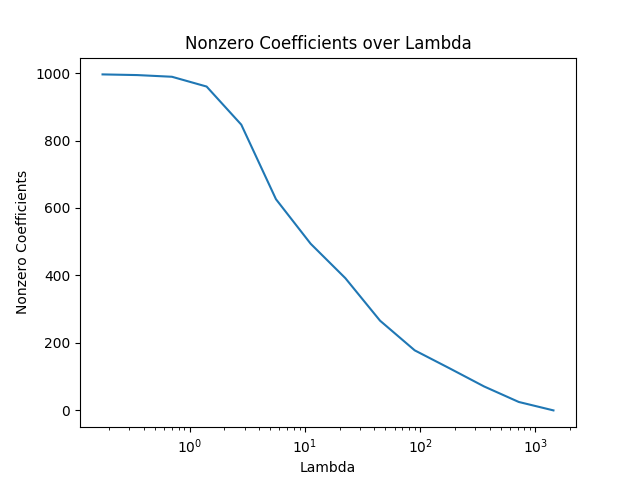
\includegraphics[width=150mm]{../hw2-code/results/a4_a.png}
\end{figure}

\subsection*{b.}

For each value of $\lambda$ tried, record values for false discovery rate (FDR) (number of incorrect nonzeros in $\widehat{w}$/total number of nonzeros in $\widehat{w}$) and true positive rate (TPR)
    (number of correct nonzeros in $\widehat{w}$/k). Note: for each $j$, $\widehat{w}_j$ is an incorrect nonzero if and only if $\widehat{w}_j \neq 0$ while $w_j = 0$.
In plot 2, plot these values with the x-axis as FDR, and the y-axis as TPR.

\begin{figure}[ht!]
  \centering
  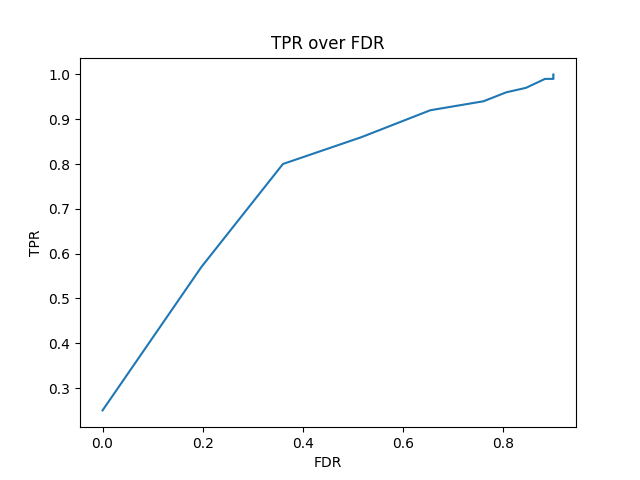
\includegraphics[width=150mm]{../hw2-code/results/a4_b.png}
\end{figure}

\subsection*{c.}

Comment on the effect of $\lambda$ in these two plots in 1-2 sentences. \\ \\
In general, having larger $\lambda$ means that we will have more zero-value weights in $w$, which makes sense since Lasso tends to encourage sparsity. We also see that larger $\lambda$ leads to lower TPR since we have fewer non-zero coefficients to err on, and thus also have lower FDR.

}

\section*{A.5}
{\Large 

\subsection*{a.}

Read the documentation for the original
  version of this dataset. Report 3 features included in this dataset for which historical \emph{policy} choices in the US would lead to variability in these features. As an example, the \emph{number of police} in a community
  is often the consequence of decisions made by governing bodies, elections, and amount of tax revenue available to decisionmakers. \\ \\
\textbf{Number of homeless people counted in the street (NumStreet):} Homeless policies and laws affecting how homeless people are treated (e.g. a notable policy where homeless people in Eastside cities like Bellevue were forcibly transported to Seattle) can affect this number. \\
\textbf{Number of people under the poverty level (NumUnderPov):} There are a lot of different factors in policy that can affect poverty statistics: varied definitions of poverty as set by institutions, whether or how benefits are provided to the impoverished, cost of living standards and how that affects wages -- the list goes on and on. \\
\textbf{Mean people per household (householdsize):} The number of people per household can vary depending on the incentives that a family might receieve within their area for having children, as well as considering other factors that might affect their willingness to have children, such as employer policies in regards to maternity or paternity leave. \\

\subsection*{b.}

Before you train a model, describe 3 features in the dataset which might, if found to have nonzero weight in model, be interpreted as \emph{reasons} for higher levels of violent crime, but which might actually be a \emph{result} rather than (or in addition to being) the cause of this violence. \\ \\
\textbf{Percentage of people 16 and over, in the labor force, and unemployed (PctUnemployed):} Unemployed people tend to be associated with crime, but one's able to become and stay employed might have been directly or indirectly affected by crime. \\
\textbf{Percentage of moms of kids 6 and under in labor force (PctWorkMomYoungKids):} Oftentimes, there is a bias against mothers who either are the breadwinners for the family or are not as present for the children leading to a tendency for their children to commit crime, however, this may not be true. \\
\textbf{Percent of people who do not speak English well (PctNotSpeakEnglWell):} People also associate immigrants or non-English speakers with crime, but this might not be accurate: these people are oftentimes those more targeted or  discriminated against when it comes to crime. \\

\subsection*{c.}

Plot the number of nonzero weights of each solution as a function of $\lambda$.

\begin{figure}[ht!]
  \centering
  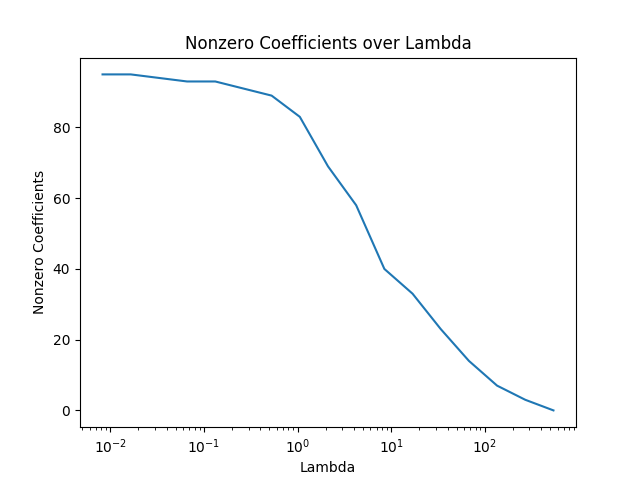
\includegraphics[width=150mm]{../hw2-code/results/a5_c.png}
\end{figure}

\subsection*{d.}

Plot the regularization paths (in one plot) for the coefficients for input variables \texttt{agePct12t29}, \texttt{pctWSocSec}, \texttt{pctUrban}, \texttt{agePct65up}, and \texttt{householdsize}.

\begin{figure}[ht!]
  \centering
  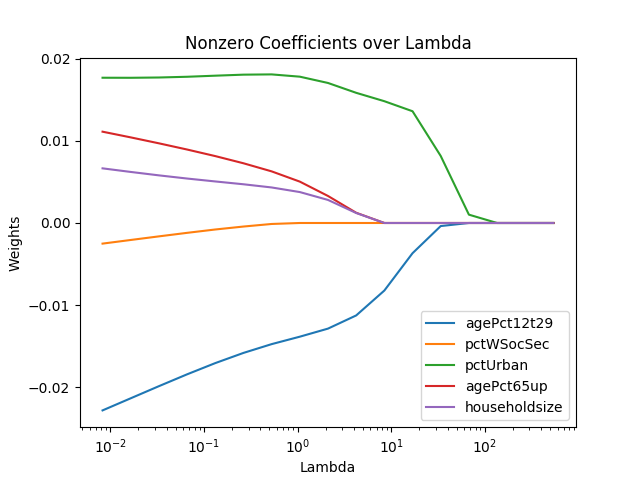
\includegraphics[width=150mm]{../hw2-code/results/a5_d.png}
\end{figure}

\subsection*{e.}

On one plot, plot the squared error on the training and test data as a function of $\lambda$.

\begin{figure}[ht!]
  \centering
  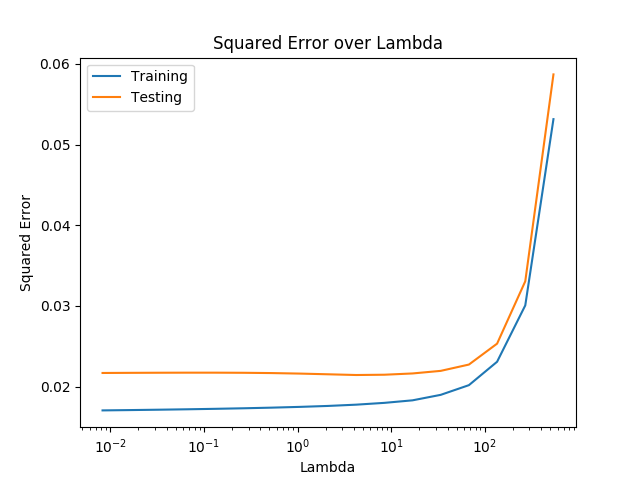
\includegraphics[width=150mm]{../hw2-code/results/a5_e.png}
\end{figure}

\subsection*{f.}

Sometimes a larger value of $\lambda$ performs nearly as well as a smaller value, but a larger value will select fewer variables and perhaps be more interpretable.  Inspect the weights $\hat{w}$ for $\lambda = 30$.  Which feature
    had the largest (most positive) Lasso coefficient? What about the most negative? Discuss briefly. \\ \\

Exact data:
\begin{verbatim}
\end{verbatim}

The most positive coefficient was found with the feature PctIlleg, which represents the percentage of kids born to never married parents. \\
The most negative coefficient was found with the feature PctFam2Par, which represents the percentage of families with 2 parents.

\subsection*{g.}

Suppose there was a large negative weight on
    \texttt{agePct65up} and upon seeing this result, a politician suggests policies that encourage people over the age of 65 to move to high crime areas in an effort to reduce crime. What is the (statistical) flaw in this line of reasoning? (Hint: fire trucks
    are often seen around burning buildings, do fire trucks cause fire?) \\ \\
The issue with this line of reasoning is that correlation implies causation, which is not necessarily true. The fact that having greater population over the age of 65 is linked to lower crime might be true, but one may not necessarily cause the other. 

}

\section*{A.6}
{\Large 

Here we consider the MNIST dataset, but for binary classification. Specifically, the task is to determine whether a digit is a $2$ or $7$.
Here, let $Y=1$ for all the ``7'' digits in the dataset, and use $Y=-1$ for ``2''.
We will use regularized logistic regression. 
Given a binary classification dataset $\{(x_i,y_i)\}_{i=1}^n$ for $x_i \in \R^d$ and $y_i \in \{-1,1\}$ we showed in class that the regularized negative log likelihood objective function can be written as
\begin{align*}
J(w,b) = \frac{1}{n} \sum_{i=1}^n \log( 1 + \exp(-y_i (b + x_i^T w))) + \lambda ||w||_2^2
\end{align*} 
Note that the offset term $b$ is not regularized. 
For all experiments, use $\lambda = 10^{-1}$. 
Let $\mu_i(w,b) = \frac{1}{1+ \exp(-y_i (b + x_i^T w))}$.

\framebox[1.1\width]{\textbf{answer}}

\subsection*{a.}

$J(w,b) = \frac{1}{n} \sum_{i=1}^n \log( 1 + \exp(-y_i (b + x_i^T w))) + \lambda ||w||_2^2$ \\
$\nabla_w J(w,b) = \nabla_w [\frac{1}{n} \sum_{i=1}^n \log( 1 + \exp(-y_i (b + x_i^T w))) + \lambda ||w||_2^2]$ \\ 
$ = \nabla_w \frac{1}{n} \sum_{i=1}^n \log( 1 + \exp(-y_i (b + x_i^T w))) + \nabla_w \lambda ||w||_2^2$ \\ 
$ = \frac{1}{n} \sum_{i=1}^n \nabla_w \log( 1 + \exp(-y_i (b + x_i^T w))) + 2 \lambda w$ \\ 
$ = \frac{1}{n} \sum_{i=1}^n \frac{1}{1 + \exp(-y_i (b + x_i^T w))} \cdot \exp(-y_i (b + x_i^T w)) \cdot -y_i (x_i^T) + 2 \lambda w$ \\ 
$ = \frac{1}{n} \sum_{i=1}^n \frac{-y_i x_i^T \exp(-y_i (b + x_i^T w))}{1 + \exp(-y_i (b + x_i^T w))} + 2 \lambda w$ \\ 
$ = \frac{1}{n} \sum_{i=1}^n -y_i x_i^T \mu_i(w, b) \exp(-y_i (b + x_i^T w)) + 2 \lambda w$ \\ 
$ = \frac{1}{n} \sum_{i=1}^n -y_i x_i^T \mu_i(w, b) (\frac{1}{\mu_i(w, b)} - 1) + 2 \lambda w$ \\ 
$ = \frac{1}{n} \sum_{i=1}^n -y_i x_i^T \mu_i(w, b) (\frac{1}{\mu_i(w, b)} - \frac{\mu_i(w, b)}{\mu_i(w, b)}) + 2 \lambda w$ \\ 
$ = \frac{1}{n} \sum_{i=1}^n -y_i x_i^T \mu_i(w, b) \frac{1 - \mu_i(w, b)}{\mu_i(w, b)} + 2 \lambda w$ \\ 
\framebox[1.1\width]{\textbf{$\nabla_w J(w,b) = \frac{1}{n} \sum_{i=1}^n -y_i x_i^T (1 - \mu_i(w, b)) + 2 \lambda w$}} \\ \\
$J(w,b) = \frac{1}{n} \sum_{i=1}^n \log( 1 + \exp(-y_i (b + x_i^T w))) + \lambda ||w||_2^2$ \\
$\nabla_{b} J(w,b) = \nabla_{b} [\frac{1}{n} \sum_{i=1}^n \log( 1 + \exp(-y_i (b + x_i^T w))) + \lambda ||w||_2^2]$ \\
$ = \nabla_{b} \frac{1}{n} \sum_{i=1}^n \log( 1 + \exp(-y_i (b + x_i^T w))) + \nabla_{b} \lambda ||w||_2^2$ \\ 
$ = \frac{1}{n} \sum_{i=1}^n \nabla_{b} \log( 1 + \exp(-y_i (b + x_i^T w))) + 0$ \\ 
$ = \frac{1}{n} \sum_{i=1}^n \frac{1}{\log( 1 + \exp(-y_i (b + x_i^T w)))} \cdot \exp(-y_i (b + x_i^T w)) \cdot -y_i(1)$ \\ 
$ = \frac{1}{n} \sum_{i=1}^n -y_i \mu_i(w, b) \cdot \exp(-y_i (b + x_i^T w))$ \\ 
$ = \frac{1}{n} \sum_{i=1}^n -y_i \mu_i(w, b) \frac{1 - \mu_i(w, b)}{\mu_i(w, b)}$ \\ 
\framebox[1.1\width]{\textbf{$\nabla_{b} J(w,b) = \frac{1}{n} \sum_{i=1}^n -y_i (1 - \mu_i(w, b))$}}

\subsection*{b.}

Implement gradient descent with an initial iterate of all zeros. Try several values of step sizes to find one that appears to make convergence on the training set as fast as possible. Run until you feel you are near to convergence.

\begin{enumerate}
  \item For both the training set and the test, plot $J(w,b)$ as a function of the iteration number (and show both curves on the same plot).
  \item For both the training set and the test, classify the points according to the rule $\text{sign}(b + x_i^T w)$ and plot the misclassification error as a function of the iteration number (and show both curves on the same plot)
\end{enumerate}

\begin{figure}[hb]
  \centering
  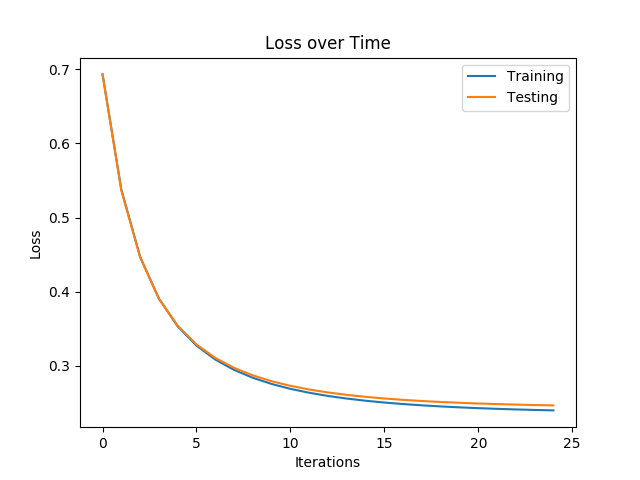
\includegraphics[width=150mm]{../hw2-code/results/a6_bi.png}
\end{figure}

\begin{figure}[hb]
  \centering
  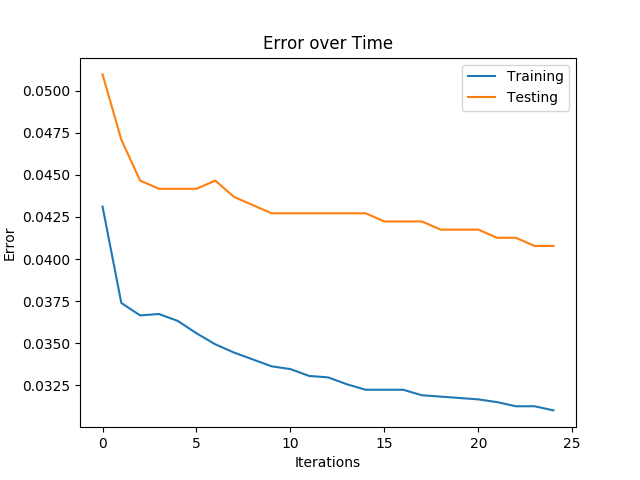
\includegraphics[width=150mm]{../hw2-code/results/a6_bii.png}
\end{figure}

\subsection*{c.}

Repeat (b) using stochastic gradient descent with a batch size of 1. Note, the expected gradient with respect to the random selection should be equal to the gradient found in part (a). Show both plots described in (b) when using batch size 1. Take careful note of how to scale the regularizer.

\begin{figure}[hb]
  \centering
  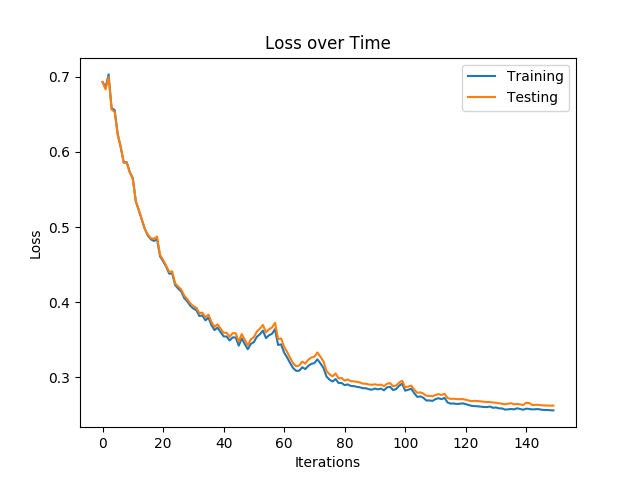
\includegraphics[width=150mm]{../hw2-code/results/a6_ci.png}
\end{figure}

\begin{figure}[hb]
  \centering
  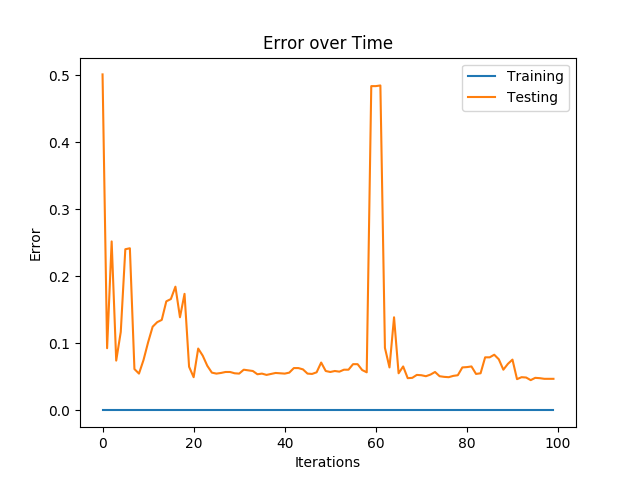
\includegraphics[width=150mm]{../hw2-code/results/a6_cii.png}
\end{figure}

\subsection*{d.}

Repeat (b) using stochastic gradient descent with batch size of 100. That is, instead of approximating the gradient with a single example, use 100. Note, the expected gradient with respect to the random selection should be equal to the gradient found in part (a).

\begin{figure}[hb]
  \centering
  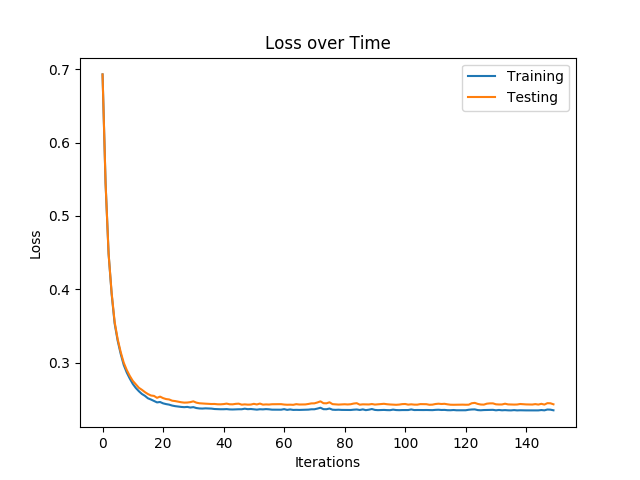
\includegraphics[width=150mm]{../hw2-code/results/a6_di.png}
\end{figure}

\begin{figure}[hb]
  \centering
  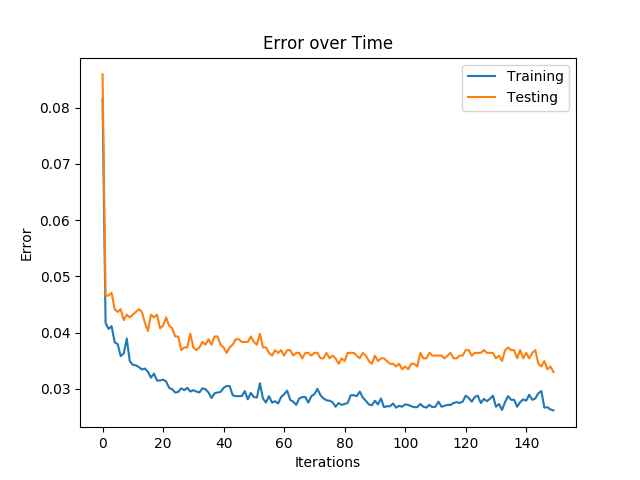
\includegraphics[width=150mm]{../hw2-code/results/a6_dii.png}
\end{figure}

}

\end{document}